\documentclass[a4paper,titlepage,12pt]{article}
\usepackage[utf8]{inputenc} %Make sure all UTF8 characters work in the document
\usepackage{listings} %Add code sections
\usepackage{color}
\usepackage{graphicx}
\usepackage{titling}
\usepackage{textcomp}
\usepackage[hyphens]{url}
\usepackage[bottom]{footmisc}
\usepackage[yyyymmdd]{datetime}
\usepackage{tikz}
\usetikzlibrary{arrows}
\definecolor{listinggray}{gray}{0.9}
\definecolor{lbcolor}{rgb}{0.9,0.9,0.9}

%Set page size
\usepackage{geometry}
\geometry{margin=3cm}
\usepackage{parskip} 

\renewcommand{\dateseparator}{-}

\author{Emil Segerbäck -- emise935
    \and
    Malcolm Vigren -- malvi108
    }


%%%%%%%%%%%%%%%%%%%%%%%%%%%%%%%
% Header and footer
%%%%%%%%%%%%%%%%%%%%%%%%%%%%%%%
\usepackage{fancyhdr}
\pagestyle{fancy}

\lhead{Malcolm Vigren, malvi108 \\
Emil Segerbäck, emise935}
\rhead{Laborationsuppgift 6}


\title{\textbf{TAOP33 -- Laborationsuppgift 6}}
\date{\today}

\begin{document}
	\maketitle
	\newpage
\section*{Beskrivning}
\section*{Modell}

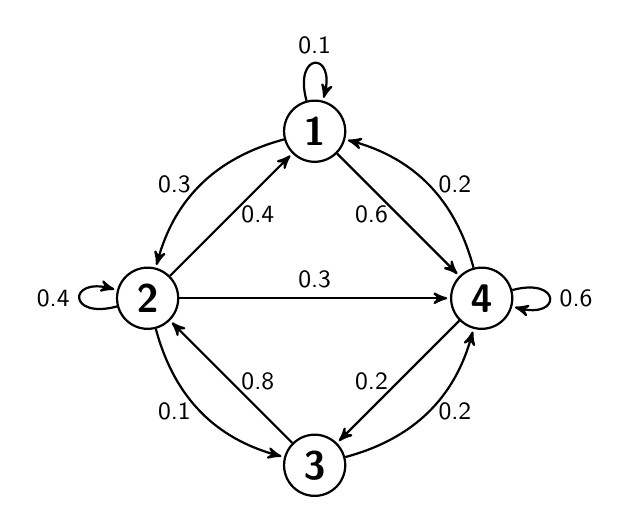
\begin{tikzpicture}[->,>=stealth',shorten >=1pt,auto,node distance=3cm,
                    thick,main node/.style={circle,draw,font=\sffamily\Large\bfseries}]

  \node[main node] (1) {1};
  \node[main node] (2) [below left of=1] {2};
  \node[main node] (3) [below right of=2] {3};
  \node[main node] (4) [below right of=1] {4};

  \path[every node/.style={font=\sffamily\small}]
    (1) edge node [left] {0.6} (4)
        edge [bend right] node[left] {0.3} (2)
        edge [loop above] node {0.1} (1)
    (2) edge node [right] {0.4} (1)
        edge node {0.3} (4)
        edge [loop left] node {0.4} (2)
        edge [bend right] node[left] {0.1} (3)
    (3) edge node [right] {0.8} (2)
        edge [bend right] node[right] {0.2} (4)
    (4) edge node [left] {0.2} (3)
        edge [loop right] node {0.6} (4)
        edge [bend right] node[right] {0.2} (1);
\end{tikzpicture}

\section*{Resultat}
\section*{Svar}
\end{document}
